\documentclass{standalone}

\usepackage{ tikz }
\usetikzlibrary{automata, positioning, arrows}

\begin{document}
    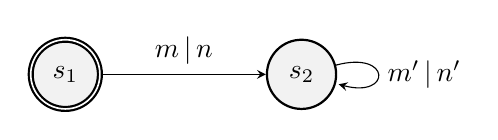
\begin{tikzpicture}[->, >=stealth, node distance=3cm, every state/.style={thick, fill=gray!10}, initial text=$ $, every edge/.append style={}]
        \node[state, accepting] (1) {$s_1$};
        \node[state, right of=1] (2) {$s_2$};

        \draw (1) edge[above] node{$m \,|\, n$} (2)
              (2) edge[loop right] node{$m^\prime \,|\, n^\prime$} (2);
    \end{tikzpicture}
\end{document}